\capitulo{4}{Técnicas y herramientas}

%Esta parte de la memoria tiene como objetivo presentar las técnicas metodológicas y las herramientas de desarrollo que se han utilizado para llevar a cabo el proyecto. Si se han estudiado diferentes alternativas de metodologías, herramientas, bibliotecas se puede hacer un resumen de los aspectos más destacados de cada alternativa, incluyendo comparativas entre las distintas opciones y una justificación de las elecciones realizadas. 
%No se pretende que este apartado se convierta en un capítulo de un libro dedicado a cada una de las alternativas, sino comentar los aspectos más destacados de cada opción, con un repaso somero a los fundamentos esenciales y referencias bibliográficas para que el lector pueda ampliar su conocimiento sobre el tema.

En esta sección se explicarán las distintas técnicas y herramientas utilizadas para llevar a cabo el proyecto.

\section{Lenguajes de programación}

\subsection{\textit{Python}}
\textit{Python} es el lenguaje de programación principal utilizado para el desarrollo de este proyecto. \textit{Python} es un lenguaje de alto nivel, interpretado, estructurado y de código abierto que puede ser usado para tareas de muchos tipos \cite{wiki:python}.

\textit{Python} se caracteriza por muchos aspectos. Y tiene múltiples ventajas respecto a otros lenguajes, como la fácil legibilidad de su código, las potentes funciones que incorpora por defecto, la utilización de tipado dinámico y las múltiples librerías de código abierto disponibles para distintas tareas, entre otras. Las ventajas que presenta respecto a otros lenguajes, como pueden ser C o Java, nos llevan a usar este lenguaje como el núcleo de nuestro proyecto.

\subsection{\textit{JavaScript}}
\textit{Javascript} es el lenguaje de programación de \textit{HTML} y de la \textit{Web}\cite{w3schools:javascript}. En nuestro caso, este es utilizado para la realización del etiquetador de imágenes, puesto que está basado en una aplicación \textit{Web}. No existen alternativas estandar a él. Pero si existen librerías para facilitar el uso del mismo, como \textit{JQuery}, la cual es utilizada en la medida de lo posible.

\subsection{\textit{JSON}}
\textit{JSON}, siglas que denotan \textit{JavaScript Object Notation}, es un formato ligero para el intercambio de datos \cite{json}. Se basa en la notación de objetos de \textit{JavaScript}, de ahí su nombre. Este es utilizado para el almacenamiento de información en nuestra aplicación, como más tarde veremos.

Existe una posible alternativa a \textit{JSON}, la cual es \textit{XML}. Este es un lenguaje de marcado que puede ser utilizado con el mismo objetivo que \textit{JSON}. Pero \textit{XML} tiene distintas desventajas respecto \textit{JSON}:

\begin{itemize}
	\item \textit{JSON} es más corto.
	\item JSON es más facil de leer.
	\item JSON se integra facilmente con \textit{Python}\footnote{Python es capaz de traducir, o \textit{parsear}, \textit{JSON} a sus propias estructuras sin que tengamos que realizar ningun paso intermedio.}.
\end{itemize}
\section{\textit{Anaconda}}

\textit{Anaconda} es un distribución de \textit{Python} y \textit{R} que facilita las tareas de gestión de paquetes, de entornos y de versiones de lenguajes de programación. Nos permite crear varios entornos con distintas versiones de paquetes o lenguajes de programación. Y nos permite la instalación, desinstalación y actualización de distintos paquetes. Facilitandonos estas tareas en la medida de lo posible.
 
\textit{Anaconda} nos provee de muchas ventajas respecto a la utilización de \textit{Python} de manera aislada. La utilización de distintas versiones del mismo lenguaje en un mismo sistema operativo es una problemática que \textit{Anaconda} nos soluciona aislandonos de todos estos problemas. Además, como previamente comentaba sobre la gestión de paquetes, \textit{Anaconda} nos provee de una herramienta, \textit{conda}, para la gestión de paquetes.

A continuación explicaré brevemente los paquetes utilizados.
 
\subsubsection{\textit{scikit-image}}

\textit{scikit-image} nos proporciona un conjunto de herramientas para el procesamiento de imágenes. En las primeras fases, fue utilizada para distintos aspectos de investigación sobre la problemática a acometer, como la segmentación de imágenes, concepto que más tarde introduciré. Pero finalmente, se utilizo únicamente para la lectura y guardado de imágenes.

%\subsection{\textit{Matplotlib}}

\subsubsection{\textit{Jupyter Notebook}}

Es una herramienta que nos permite crear \textit{webs} interactivas con código, texto, representaciones de los datos o distintas visualizaciones, como imágenes. Muchos de los productos generados por este proyecto serán de este tipo, como el etiquetador de imágenes que más tarde introduciré.

\subsection{Gestor de tareas: \textit{ZenHub}}

\textit{ZenHub} es una herramienta para la gestión de proyectos totalmente integrada con \textit{GitHub}. Esta herramienta nos permite obtener diagramas \textit{burndown}\footnote{Un diagrama \textit{burndown} es un gráfico que representa la cantidad de trabajo restante.} utilizados en el anexo de planificación del proyecto para el seguimiento del proyecto, véase la figura \ref{fig:4.2.1}. También nos permite obtener un gráfico en el que podemos ver los puntos de historia\footnote{Los puntos de historia es una medida del esfuerzo a realizar para completar una tarea.} en los distintos \textit{sprints}\footnote{\textit{Sprint} es un periodo de tiempo en el que el conjunto de las tareas, definidas al principio de este, deben ser finalizadas y revisadas.}. Y, finalmente, nos proporciona un tablero \textit{kanban} para mejorar el flujo de trabajo.

\begin{figure}[h]
\centering
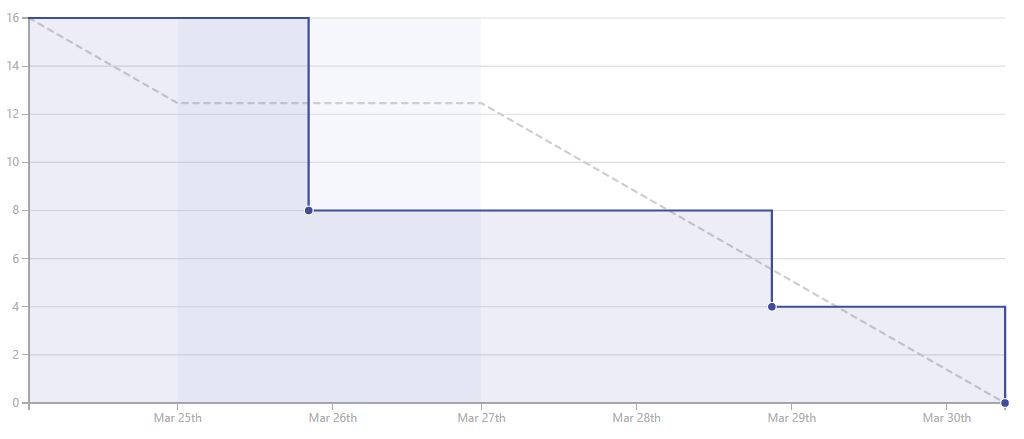
\includegraphics[width=0.99\textwidth]{sprint_7}
\caption{Ejemplo de diagrama \textit{burndown} de un  \textit{sprint}}
\label{fig:4.2.1}
\end{figure}

\section{Control de versiones: \textit{Git}}

El control de versiones es una parte fundamental para la realización de un proyecto. Este nos permite acometer distintas acciones, como comprobar el cambio realizado entre versiones, trabajar en equipo facilmente o volver a un punto anterior, entre otras cosas. En nuestro caso, utilizamos \textit{Git} como control de versiones. 

\textit{Git} nos proporciona las características que necesitamos. Además de algunas ventajas respecto a otras herramientas, como ser un sistema distribuido o proporcionar una interfaz de comandos muy potente.

%Y, además, tenía una experiencia básica con la herramienta. Lo cual, facilitaba la adopción de esta como herramienta de control de versiones.

\section{Repositorio: \textit{Github}}

Otra herramienta principal, a seleccionar, es el repositorio central, en nuestro caso hemos elegido \textit{Github}. \textit{Github} nos proporciona muchas utilidades y una forma simple de llevar a cabo el proyecto con todas las características necesarias. Es por todas sus características y una previa experiencia con la herramienta por lo que se eligió como nuestro servicio de repositorio central.

\section{Librerías auxiliares}

Para llevar a cabo este proyecto, además de las librerías ya citadas, se han utilizado algunos repositorios auxiliares para llevar a cabo algunas de las tareas. Indico a continuación los repositorios con una breve descripción:

\begin{itemize}
	\item \textit{Jupyter Dashboards}: es una extensión que nos permitirá mostrar un \textit{Jupyter Notebook} con un estilo más personalizado.
	\item \textit{IPython File Upload}: es una extensión que nos permitirá subir imágenes desde un \textit{Jupyter Notebook}.
	\item \textit{darkflow}: es una implementación de \textit{YOLO}, concepto que más tarde introduciremos, utilizado para el reconocimiento automático de fitolitos.
\end{itemize}

\section{Documentación: \LaTeX}

La memoria y anexos de este proyecto han sido escritos en \LaTeX. Este nos proporciona muchas ventajas en contraste con otros editores de documentos, como \textit{Word} o sus alternativas, a la hora de realizar un documento de estas características.

\LaTeX\ nos facilita concentrarnos simplemente en el contenido. Supeditando a este la problemática de como debe formatearse el contenido. Por lo tanto, \LaTeX\ automatiza muchas de las típicas tareas que llevaríamos a cabo con otro editor de documentos y, además, permite obtener documentos con una altísima calidad.

\section{Entorno de desarrollo: \textit{JetBrains PyCharm}}

El entorno de desarrollo o, por sus siglas \textit{IDE}, es la aplicación utilizada para el desarrollo de la aplicación. Proporcionando múltiples herramientas, desde el auto-completar, hasta \textit{plugins} que permiten comprobar el recubrimiento del código mediante tests, entre otras funcionalidades.

Para esta utilidad se valorarón dos herrramientas principalmente: \textit{PyDev} y \textit{JetBrains PyCharm}. Escogiéndose esta última por poseer una mayor cantidad de herramientas integradas, como el control de versiones, distintas opciones para refactorizar el código y un muy buen auto-completar, entre otras características.

\section{Herramienta de prototipado: \textit{NinjaMock}}

La herramienta de prototipado es la aplicación utilizada para un primer diseño de la interfaz de una aplicación. Facilitando la demostración, evaluación y agilizando el proceso de llevar a cabo una interfaz. En nuestro caso se utilizo \textit{NinjaMock}, la cual es una aplicación web que nos permite llevar a cabo esta tarea facilmente.